\documentclass[12pt,a4paper]{article}
\usepackage{better_poster}


% ---- fill in from here

% authors
\title{Chci pomáhat v rozvoji fakulty v prospěch studentú i akademické obce}
\author{Lana Sinapayen, Someone Else}

% type of poster: [exp]erimental results, [methods], [theory]
% Disclaimer: the original classification had "study" and "intervention" as separate categories. I group them under experimental results.
\newcommand\postertype{exp} % [exp],[methods],[theory]

\begin{document}

% main point of your study
\makefinding{
%\textbf{Martin Ladecký}\\
kandidát č.\textbf{14.} \\
do studentské komory\\
AS FSV ČVUT 
}


% \makemain{
% }{

% }


% the main text of your poster goes here
\makemain{
    % you can have 1 or 2 columns
    \raggedcolumns
    \begin{multicols}{2}
        \section{Intro}
        \begin{itemize}
        \setlength\itemsep{0.1em}
            \item 
            \item No need to cite papers
            \item because people can download your paper
        \end{itemize}
        
        \section{Methods}
        \begin{itemize}
        \setlength\itemsep{0.1em}
            \item N = 30
            \item Collected this
            \item Tested with X statistical test
        \end{itemize}
  %%%      
    % this determines where your columns will be separated
    \columnbreak

        \section{Results}
        
        
\includegraphics[width=\linewidth]{icons8-ecg-96.png}
        \begin{itemize}
        \setlength\itemsep{0.1em}
            \item Your
            \item Talking
            \item Points
        \end{itemize}
    
    \end{multicols}
}
% If you have extra figures or data to show
\makeextracolumn{
    Add your things here
    
    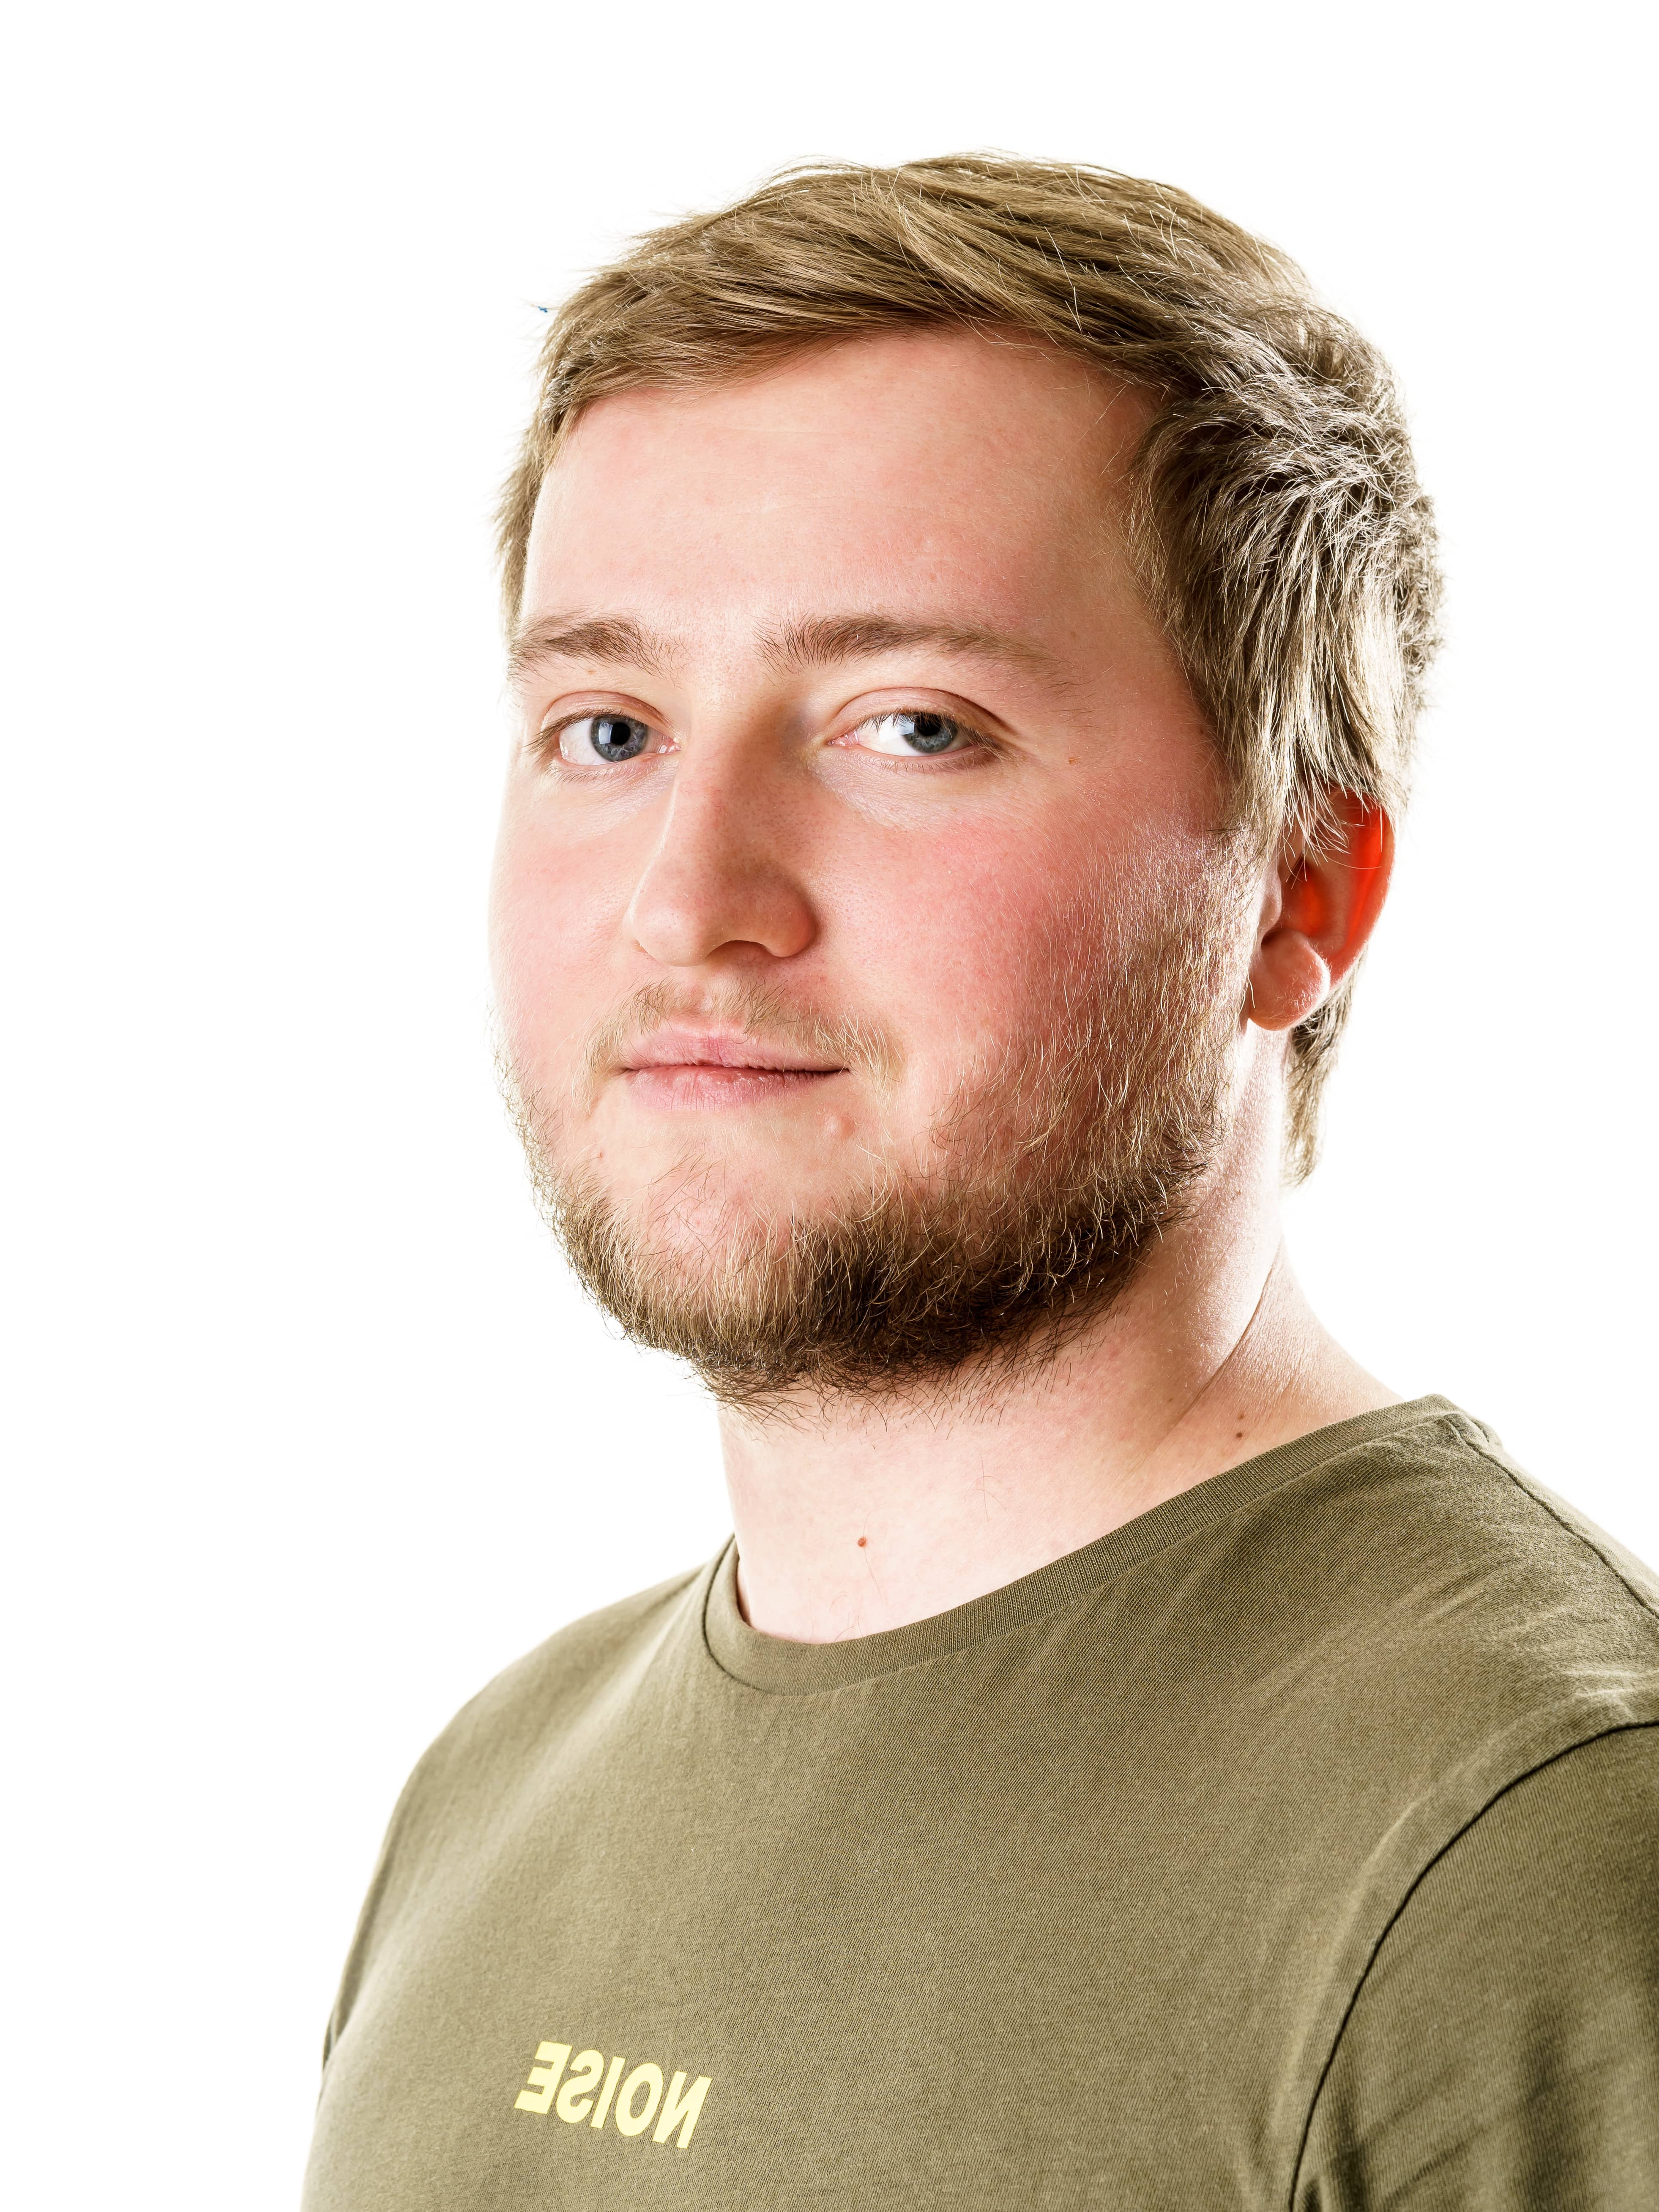
\includegraphics[width=1\linewidth]{images/photo_ML.jpg}
  %  \includegraphics[width=0.5\linewidth]{}
    
    \begin{itemize}
    \setlength\itemsep{0.1em}
        \item doktorand
        \item 
    \end{itemize}
}

% footer
% generate qr code from https://www.qr-code-generator.com/ and replace qr_code.png
% default: barcode on the left
\makefooter{images/uni_logo.png}{images/symbol_cvut_plna_verze.jpg}

% replace with this like for barcode on the right
%\makealtfooter{images/uni_logo.png}{images/qr-code.png}
 
\end{document}